\documentclass[12pt,a4paper]{report}
\usepackage[spanish, es-noindentfirst]{babel}
\selectlanguage{spanish}
\usepackage[utf8]{inputenc} 
\usepackage{animate}
% ajusta tus márgenes de página aquí
\usepackage[top=0.70in, bottom=0.70in, left=0.8in,right=0.80in]{geometry} 
% configurando la alineación de la página con este paquete
\usepackage[pdftex]{graphicx} % para incrustar imágenes
\usepackage[%dvips, % commented for pdflatex
bookmarks,  colorlinks=false]{hyperref}% para crear enlaces en la versión en pdf y otros atributos pdf adicionales, sin efecto en el documento impreso
\usepackage[table]{xcolor}
\hypersetup{%
    pdfborder = {0 0 0}
}
\usepackage[final]{pdfpages} % para incrustar otro pdf, eliminar si no es necesario
\usepackage{float} %used for figure placement with H as a parameter
\usepackage{hyperref}
\usepackage{pslatex} % for times new roman, old package, but works
\usepackage{array} % for making text bold in table
\usepackage{setspace}
\usepackage{float}
\usepackage{enumerate}
\usepackage{longtable}

\usepackage[font=small,labelfont=bf]{caption}
\def\figurename{\textbf{Figure }}

\usepackage{listings}% esto es por si se utiliza código (java, python, etc)
% Para el encabezado y el pie de página
\usepackage{fancyhdr}
\fancypagestyle{plain}{%
\fancyfoot[L]{\emph{Equipo1}}% excepto el centro
\fancyfoot[R]{\thepage}
\renewcommand{\headrulewidth}{0.4pt}
\renewcommand{\footrulewidth}{0.4pt}
}

\pagestyle{fancy}

\rhead{\emph{Plan para la dirección del proyecto}}

\fancyfoot[LO,LE]{\emph{Equipo1}}
\cfoot{}
\fancyfoot[RO, RE]{\thepage}
\renewcommand{\headrulewidth}{0.4pt}
\renewcommand{\footrulewidth}{0.4pt}


%Borde de página
\usepackage{pgf}
\usepackage{pgfpages}

\begin{document}
\renewcommand\bibname{References}
\lhead{ }

\newpage
\
%Portada
\setlength{\unitlength}{1 cm} %Especificar unidad de trabajo
\thispagestyle{empty}
\begin{picture}(18,4)
\put(0,0){
\includegraphics[width=4cm,height=4cm]{project/images/uib.png}}
\put(11.5,0.4){\animategraphics[autoplay,loop,width=3.5cm,height=3.5cm]{6}{project/logo/logo_}{0}{6}}
\end{picture}
\\
\\
\begin{center}
\textbf{{\Huge Universidad de Las Islas Baleares}\\[0.5cm]
{\LARGE Escuela Politécnica Superior}}\\[1.25cm]
{\Large Proyectos}\\[2.3cm]
{\LARGE \textbf{Plan para la dirección de proyecto}}\\[3.5cm]
{\large Arbós Parets, Pere}\\[0.5cm]
{\large Ladó Salas, Carlos}\\[0.5cm]
{\large Nolasco Pajuelo, Kevin Alexander Jhosep}\\[0.5cm ]
{\large Orellana Rodriguez, Gary}\\[2cm]
\today
\end{center}
\newpage

%TABLE OF CONTENTS AND LIST OF FIGURES ARE AUTOMATICALLY ADDED BY FOLLOWING COMMANDS
%ADD FIGURE OF TABLES IF YOU NEED TO, CHECK DOCUMENTATION
\pagenumbering{roman} %numbering before main content starts


%To reset the Header & Footer for TOC and LOF
\pagestyle{empty}
\addtocontents{toc}{\protect\thispagestyle{empty}}
\tableofcontents %  agregar el índice

\addtocontents{lof}{\protect\thispagestyle{empty}}
\listoffigures % agregar lista de imágenes
\listoftables
\cleardoublepage

%And reset back the settings we choose for Header and Footer
\pagestyle{fancy}

\newpage
\pagenumbering{arabic} %reset numbering to normal for the main content

\chapter{Gestión de alcance}



\section{Objetivos del proyecto}
El objetivo del proyecto consta de la realización de una instalación ICT en un bloque de cinco plantas. La instalación estará formada por RTV, fibra óptica, televisión por cable y par trenzado. Entregaremos la instalación cuando se cumpla con todos los requisitos y obligaciones del Real Decreto 346/2011.

\section{Descripción del alcance del producto}
La instalación se realizará en un bloque de cinco pisos, constituido por un local en la planta inferior y cuatros plantas superiores. Esta instalación se llevará a cabo por dos instaladores de nuestra empresa. Éstos deberán instalar el cableado de canalización exterior, de enlace, principal, secundaria e interior del usuario. El diseño de las canalizaciones se hará a petición del cliente. A continuación se describirán los productos necesarios para cada instalación.
\begin{itemize}
\item \textbf{Instalación de RTV:} se necesitará cable coaxial, tomas RTV, amplificadores de señal, derivadores (por lo menos de tres tipos), repartidores y antenas(TV, FM y DAB); las antenas satélites quedan excluidas por petición del cliente.
\item \textbf{Instalación CATV:} se necesitará cable coaxial, un panel de distribución y tomas CATV.
\item \textbf{Instalación STDP:} se necesitará cable de par trenzado UTP de categoría 6 (por petición del cliente), un panel de distribución, roseta de terminación, multiplexores y tomas RJ-45.
\item \textbf{Instalación fibra óptica:} se necesitarán cable de fibra óptica sc/apc, panel de distribución y caja de conexiones.
\end{itemize}
Todas estas instalaciones se realizarán con los instrumentos necesarios y cumpliendo con la normativa y los requisitos del cliente.

\section{Requisitos del proyecto}
Tras mantener varias reuniones con el cliente, a continuación citaremos los requisitos pedidos:
\begin{itemize}
\item [$-$] Disponemos de 3 meses para realizar el proyecto.
\item [$-$] Debemos realizar la instalación completas de RTV, CATV y STDP.
\item [$-$] La instalación de fibra óptica se hará hasta cada PAU, por si en un futuro es necesario y solo se hará la instalación interior del usuario.
\item [$-$] NO  realizaremos la instalación de TVSat.
\item [$-$] Instalaremos el mínimo de tomas que debe haber en cada vivienda de un bloque de 5 PAUs. Este mínimo de tomas se especifica en la normativa.
\item [$-$] En la fecha de entrega, otorgaremos la instalación certificada por su buen funcionamiento y con dos manuales de usuario, uno en castellano y otro en catalán.
\item [$-$] El diseño de la canalización principal y secundaria se realizará, a petición del cliente, en el momento de la instalación.
\item [$-$] Los embellecedores de las tomas se escogerán por parte del cliente.
\item [$-$] La calidad de los materiales de la instalación (cables, distribuidores, etc.) serán de gama alta.
\end{itemize}
\section{Entregables}
Los entregables del proyecto serán los siguientes:
\begin{itemize}
\item La instalación ICT acabada.
\item El boletín del protocolo de pruebas.
\item Los manuales de usuario, uno en castellano y otro en catalán.
\item El documento de fin de obra.
\end{itemize}
\section{Criterios de Aceptación}
El proyecto será aceptado por el cliente si:
\begin{itemize}
\item [$-$] Todas las instalaciones a realizar están acabadas y funcionan correctamente.
\item[$-$] Todos los requisitos del cliente se cumplan. 
\end{itemize}
\section{Suposiciones del proyecto}
El edificio en el que realiza la ICT, damos por supuesto que es un edificio ordinario en el sentido de que no presente irregularidades que dificulten o supongan un problema para la instalación.
\section{Riesgos iniciales}
El riesgo inicial más importante que tenemos es que el presupuesto debe ser suficiente para realizar el proyecto. En caso de que el presupuesto no sea suficiente, nos vemos obligados a usar material de gama media e ignorar los embellecedores de toma o el diseño indicado a petición del cliente y, en su lugar, proporcionar unos de menor presupuesto que se puedan permitir para que la instalación pueda finalizar correctamente. \\
Otro riesgo inicial es que fallemos en los cálculos preliminares y, a causa de esto, tengamos niveles de toma con una relación señal/ruido regular. Para evitar esto, iremos realizando cálculos preliminares de forma periódica mientras se ejecuta la instalación. También corremos el riesgo de que el cliente cambie o añada requisitos.
\section{Estructura Desglosada del Trabajo del proyecto (EDT)}
A continuación se muestra la EDT por fases del proyecto:
\begin{figure}[H]
\centering
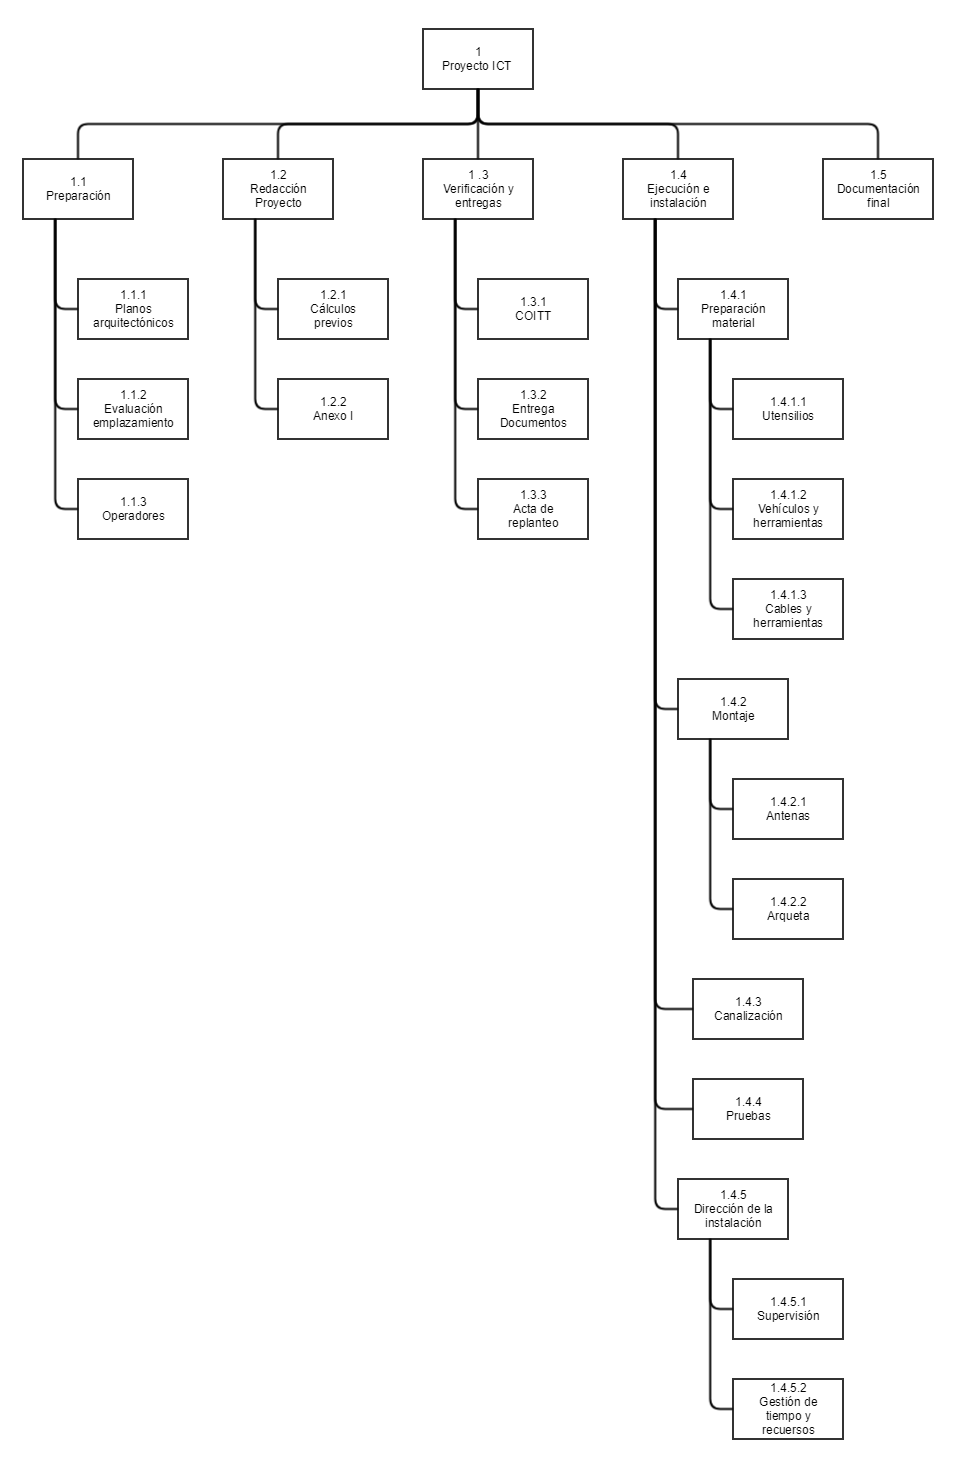
\includegraphics[scale = 0.55]{project/images/edt.png}
\caption{Estructura EDT}
\end{figure}
%%%%%%%%%%%%%%%%%%%%%%%%%%%%%%%%%%%%%%%%%%%%%%%%%%%%%%%%%%%%%%
%Aquí esta el diccionario, sobre la posición me daba errores no lo se porque bueno, una vez acabado se verá sobre la posición por ahora rellenar esto y luego haremos cambios, es fácil entender esta tabla así que no creo que tengan problemas.
%\newgeometry{left = 1.5cm,right = 1cm}
\begin{table}[H]
\begin{tabular}{|m{1cm}|m{2cm}|m{5cm}|m{2cm}|m{2.5cm}|m{2.8cm}| }
\hline
 \multicolumn{6}{|c|}{\centering Diccionario} \\
\hline
\rowcolor{gray!50}  \centering EDT código & \centering Código (EDT) & Actividades y Definición & Responsables & Fecha & Dependencias \\
\hline
  \centering 1\\ (nv 1) & \centering Proyecto ICT & Se realizará una proyecto para implementar una ICT. & \centering Director &Inicio: 18/12/17 Fin: 18/03/19& Ninguna \\
\hline
  \centering 1.1\\ (nv 2) & \centering Preparación & Preparar los documentos y mantener comunicaciones previas  a  la redacción del proyecto \. & \centering Director de obra &Inicio: 18/12/17 Fin: 18/01/18 & Antes de (1.2) \\
\hline
 \centering 1.1.1\\ (nv 3) & \centering Planos arquitectónicos & (A) Comunicarse con el Arquitecto para facilitar los planos en fase de final de la obra. & \centering  Director &Inicio: 18/12/17 Fin: 18/12/17 & Antes de (1.1.2)\\
\hline
 \centering 1.1.2\\ (nv 3) & \centering Evaluación emplazamiento &  Observación de la ubicación: (A) Observar edificios del alrededor para cálculo de sombra radioeléctrica; (B) Observar si hay existencia de dotación de servicios; (C) Evaluar el estado de las redes de telecomunicación de la zona; (D) Obtener medidas de potencia de señal. & \centering Ingenieros e Instaladores &Inicio: 19/12/17 Fin: 23/12/17 & Después de (1.1.1) \\
\hline
 \centering 1.1.3\\ (nv 3) & \centering Operadores & (A) Consultar de forma telemática con los operadores para definir qué redes no se van a implementar.& \centering Jefe de proyecto &Inicio: 18/12/17 Fin: 18/01/18 & Ninguna\\
\hline
\centering 1.2\\ (nv 2) & \centering Redacción proyecto & Fase de redacción del proyecto de ICT. & \centering Jefe de proyecto &Inicio: 24/12/17 Fin: 18/01/18& Después de (1.1) Antes de (1.3)\\
\hline
 \centering 1.2.1\\ (nv 3) & \centering Cálculos previos & (A) Elección del tipo de cableado, (B) Realizar propósito de distribución similar de los niveles de atenuación y de señal, esquema de red, elementos y dimensión de RTV, planos de infraestructura y (C) Colocar de la arqueta de entrada sobre el plano. & \centering Ingenieros &Inicio: 25/12/17 Fin:30/12/17& Después de 1.1.2\\
\hline
 \centering 1.2.2\\ (nv 3) & \centering Anexo I & (A) Rellenar según el Anexo I. & \centering Jefe de Proyecto &Inicio: 26/12/17 Fin: 18/01/18& Ninguna\\
\hline
 \centering 1.3\\ (nv 2) & \centering Verificación y entregas & Trámites de verificación y entregas que se deben realizar del proyecto. & \centering Director &Inicio: 19/01/18 Fin: 27/01/18& Después de (1.2) Antes de (1.4) \\
\hline
 
\end{tabular}
%Lo que sigue lo pueden quitar si lo desean, no sabía si al final habra que hacer como un lugar especial donde irán todas las tablas

\caption{Diccionario del EDT 1}
\label{table:ta}
\end{table}
\begin{table}[H]
\begin{tabular}{|m{1cm}|m{2cm}|m{5cm}|m{2cm}|m{2.5cm}|m{2.8cm}| }
\hline
 \multicolumn{6}{|c|}{\centering Diccionario} \\
\hline
\rowcolor{gray!50} \centering EDT código & \centering Código (EDT) & Actividades y Definición & Responsables & Fecha & Dependencias \\
\hline
\centering 1.3.1\\ (nv 3) & \centering COITT & (A) Entregar el proyecto al Colegio Oficial de Ingenieros Técnicos de Telecomunicación. (B) Recibir verificación. & \centering Director &Inicio: 19/01/18 Fin: 26/01/18 & Ninguna\\
\hline
 \centering 1.3.2\\ (nv 3) & \centering Entrega documentos & (A) Entregar una copia del proyecto a la Propiedad. (B) Entregar una copia del proyecto al Ministerio. & \centering Director & Inicio: 26/01/18 Fin: 27/01/18& Ninguna\\
\hline
 \centering 1.3.3\\ (nv 3) & \centering Acta de replanteo & (A) Redactar el acta de replanteo. (B) Entregar acta de replanteo. & \centering Director de obra & Inicio: 26/01/18 Fin: 27/01/19& Después de (1.3.2), antes de (1.4.1), (1.4.2), (1.4.3) y(1.4.4).\\
\hline
\centering 1.4\\ (nv 2) & \centering Ejecución e instalación & Procesos de ejecución e instalación en la infraestructura en la que se realiza el proyecto ICT. & Director e Ingenieros & Inicio: 27/01/18 Fin: 10/03/19& Después de (1.3) \\
\hline
 \centering 1.4.1\\ (nv 3) & \centering Preparación material & Preparación el material que se utilizará para la instalación del proyecto.& Instaladores & Inicio: 27/01/19
 Fin: 29/01/19& Antes de (1.4.2)\\
\hline
 \centering 1.4.1.1\\ (nv 4) & \centering Utensilios & (A) Preparación de los utensilios. (B) Presentación de los utensilios en el edificio. & Instaladores & Inicio: 27/01/19 Fin:28/01/19& Ninguna \\
\hline
 \centering 1.4.1.2\\ (nv 4) & \centering Vehículos y herramientas & (A) Preparación de vehículos y herramientas. (B) Presentación de vehículos y herramientas en el edificio. & Instaladores & Inicio: 27/01/19 Fin:29/01/19& Ninguna \\
\hline
 \centering 1.4.1.3\\ (nv 4) & \centering Cables y canalización & (A) Preparación del cableado. (B) Presentación del cableado en el edificio. & Instaladores & Inicio: 27/01/19 Fin: 29/01/19 & Ninguna \\
\hline
 \centering 1.4.2\\ (nv 3) & \centering Montaje & Fase de montaje de las infraestructuras del proyecto.& Instaladores & Inicio: 29/01/19 Fin: 18/02/19& Después de (1.4.1) Antes de (1.4.3) \\
\hline
 \centering 1.4.2.1\\ (nv 4) & \centering Antenas &
(A) Montaje de antenas. & Instaladores & Inicio: 29/01/19 Fin: 18/02/19& Ninguna \\
 \hline
 \centering 1.4.2.2\\ (nv 4) & \centering Arqueta &
 (A) Montaje de la arqueta de entrada. (B) Conectividad de la arqueta de entrada. & Instaladores & Inicio: 29/01/19 Fin: 18/02/19 & Ninguna \\
\hline
 \centering 1.4.3\\ (nv 3) & \centering Canalización & 
(A) Instalación del cableado. (B) Montaje de los embellecedores. & Instaladores & Inicio: 19/02/19 Fin: 03/03/19 & Después de (1.4.2) Antes de (1.4.4) Antes de (1.5) \\
\hline
 
\end{tabular}
%Lo que sigue lo pueden quitar si lo desean, no sabía si al final habra que hacer como un lugar especial donde irán todas las tablas
\caption{Diccionario del EDT 2}
\label{table:ta1}
\end{table}
\begin{table}[H]
\begin{tabular}{|m{1cm}|m{2cm}|m{5cm}|m{2cm}|m{2.5cm}|m{2.8cm}| }
\hline
 \multicolumn{6}{|c|}{\centering Diccionario} \\
\hline
\rowcolor{gray!50} \centering EDT código & \centering Código (EDT) & Actividades y Definición & Responsables & Fecha & Dependencias \\
\hline
 \centering 1.4.4\\ (nv 3) & \centering Pruebas & 
 (A) Realización de pruebas del funcionamiento de la instalación. & Ingenieros & Inicio: 04/03/19 Fin: 10/03/19 & Después de (1.4.3)\\
\hline
 \centering 1.4.5\\ (nv 3) & \centering Dirección de la Instalación & El proceso de instalación se debe supervisar para que transcurra según lo planeado. También hay que gestionar los imprevistos en la administración del tiempo y las posibles faltas de recursos.& \centering Director & Inicio: 27/01/18 Fin: 10/03/19 & Durante (1.4) \\
\hline
 \centering 1.4.5.1\\ (nv 4) & \centering Supervisión & 
(A) Comprobación de proceso de instalación. (B) Resolución de dudas. (C) Resolución de conflictos. & \centering Director e Ingenieros& Inicio: 27/01/18 Fin: 10/03/19 & Ninguna \\
 \hline
 \centering 1.4.5.2\\ (nv 4) & \centering Gestión de tiempo y recursos & (A) Reajustes de planificación temporal. (B) Reajustes de presupuesto. & \centering Director y Jefe de proyecto & Inicio: 27/01/18 Fin: 10/03/19 & Ninguna \\
\hline
 \centering 1.5\\ (nv 2) & \centering Documentos finales & (A) Realizar boletín de instalación.
(B) Realización de protocolos de prueba.
(C) Realización de manual de usuario. & \centering Director & Inicio: 11/03/19 Fin: 18/03/19 & Después de (1.4.3) \\
\hline
\end{tabular}
\caption{Diccionario del EDT 3}
\label{table:ta1}
\end{table}

%%%%%%%%
\subsection{Hitos}

\begin{itemize}

\item Inicio del proyecto - Inicio de (1).
\item Completar la redacción del proyecto - Fin de (1.2).
\item Verificación del proyecto - Fin de (1.3.1).
\item Inicio de la instalación - Inicio de (1.4).
\item Terminar el proceso de montaje e instalación - Fin de (1.4.3).
\item Finalización del proyecto - Fin de (1).

\end{itemize}
%%%%%%%
\newpage
 
\chapter{Gestión del tiempo}
%\paragraph{}WRITE HERE

\section{Descripción de actividades}


\subsection{Obtención de planos arquitectónicos}
\begin{itemize}
\item \textbf{Identificador: }1.1.1 A.
\item \textbf{Paquete de trabajo: }Planos arquitectónicos.
\item \textbf{Descripción: }Mediante una citación telemática o telefónica, se concierta una reunión con el Arquitecto de la edificación. En dicha reunión se obtendrán los planos arquitectónicos del edificio en fase de finalización de obra, dado que en esta fase no se modificará la edificación y se podrá ejecutar la instalación de la ICT.
\item \textbf{Responsable: }Director.
\item \textbf{Requisitos de recursos: }
\item \textbf{Estimación de duración: }1 día.
\item \textbf{Secuencia de actividades: }Esta actividad no necesita de otra para ser iniciada, sino que es la primera actividad de la que procederán los siguientes paquetes de trabajo.
\end{itemize}

\subsection{Álex1}
\begin{itemize}
\item \textbf{Identificador: }
\item \textbf{Paquete de trabajo: }
\item \textbf{Descripción: }
\item \textbf{Responsable: }
\item \textbf{Requisitos de recursos: }
\item \textbf{Estimación de duración: }
\item \textbf{Secuencia de actividades: }
\end{itemize}

\subsection{Álex2}
\begin{itemize}
\item \textbf{Identificador: }
\item \textbf{Paquete de trabajo: }
\item \textbf{Descripción: }
\item \textbf{Responsable: }
\item \textbf{Requisitos de recursos: }
\item \textbf{Estimación de duración: }
\item \textbf{Secuencia de actividades: }
\end{itemize}

\subsection{Obtener medidas de potencia de señal}
\begin{itemize}
\item \textbf{Identificador: }1.1.2 D.
\item \textbf{Paquete de trabajo: }Evaluación de emplazamiento.
\item \textbf{Descripción: }Vamos a la ubicación, donde se va a realizar el proyecto, evaluamos todos aspectos necesarios para realizar los cálculos previos, uno de estos aspectos es obtener las medidas de potencia de señal. Medimos la potencia de señal recibida en varios puntos del emplazamiento y estudiaremos cuál es el mejor sitio para colocar las antenas de la instalación RTV.
\item \textbf{Responsable: }Ingenieros y los instaladores.
\item \textbf{Requisitos de recursos: }Para esta actividad será necesario un medidor de radiación electromagnética para observar la calidad de señal recibida y sus interferencias. Los ingenieros escogerán 5 lugares, previamente estudiados, para medir. Los instaladores realizarán las medidas en dichos puntos.
\item \textbf{Estimación de duración: }3-4 días.
\item \textbf{Secuencia de actividades: }Para hacer esta actividad es necesario que se haya obtenido los planos arquitectónicos(paquete de trabajo 1.1.1). Tras esta actividad, ya se puede hacer los cálculos previos (paquete de trabajo 1.2.1).
\end{itemize}

\subsection{Entregar el proyecto a una entidad verificadora}
\begin{itemize}
\item \textbf{Identificador: }1.3.1 A.
\item \textbf{Paquete de trabajo: }COITT.
\item \textbf{Descripción: }El director de obra entregará el proyecto a una entidad verificadora, como el  Colegio Oficial de Ingenieros Técnicos en Telecomunicaciones(COITT). Esta entidad irá informando si hay que realizar cambios en el proyecto y,finalmente, dará respuesta si el proyecto es verificado o no.
\item \textbf{Responsable: }Director de obra.
\item \textbf{Requisitos de recursos: }Es necesario tener redactado el proyecto.
\item \textbf{Estimación de duración: }
\item \textbf{Secuencia de actividades: }Esta actividad se realiza cuando se haya acabado de redactar el proyecto(paquete de trabajo 1.2). Tras esta actividad se puede proceder a la ejecución e instalación(paquete de trabajo 1.4).
\end{itemize}

\subsection{Instalación del cableado}
\begin{itemize}
\item \textbf{Identificador: }1.4.3 A.
\item \textbf{Paquete de trabajo: }Instalación del cableado.
\item \textbf{Descripción: }...
\item \textbf{Responsable: }Instaladores.
\item \textbf{Requisitos de recursos: }... 
\item \textbf{Estimación de duración: }...
\item \textbf{Secuencia de actividades: }Esta actividad viene precedida de la tarea 1.4.2. Tras esta actividad, se realizarán los paquetes 1.4.4 y 1.5.
\end{itemize}

\subsection{Resolver dudas en el proceso de intalación}
\begin{itemize}
\item \textbf{Identificador: }1.4.5.1 B.
\item \textbf{Paquete de trabajo: }Supervisión.
\item \textbf{Descripción: }Los ingenieros estarán presentes en el proceso de instalación para resolver las dudas que puedan surgirles a los instaladores. El director visitará la obra periódicamente (dos veces a la semana) por si su ayuda fuese necesaria. En caso de requerir la opinión del cliente para ciertos aspectos del montaje de la instalación, será el director el encargado de comunicarse con este para conocer sus criterios y preferencias.
\item \textbf{Responsable: }Director e Ingenieros.
\item \textbf{Requisitos de recursos: }Ninguno (la presencia de los responsables en el lugar de la instalación es suficiente).
\item \textbf{Estimación de duración: }7 semanas.
\item \textbf{Secuencia de actividades: } Esta actividad debe realizarse simultáneamente al proceso de instalación, lo que representa el conjunto de todas las actividades de (1.4).
\end{itemize}

\subsection{Realización del manual de usuario}
\begin{itemize}
\item \textbf{Identificador: }1.5 C.
\item \textbf{Paquete de trabajo: }Documentos finales.
\item \textbf{Descripción: }El director, con ayuda del jefe de proyecto si fuese necesario, redactará el manual de usuario de la ICT que se ha realizado, siguiendo las indicaciones del Anexo VI de la Orden ITC/1644/2011. Dicho manual deberá incluir:
\begin{enumerate}
\item Identificación del edificio
\item Objetivo del documento
\item Introducción
\item Esquema de la instalación efectuada
\item Resumen de servicios instalados
\item Descripción de la instalación interior de usuario
\item Servidumbres
\item Garantía de la ICT
\item Documentación de las Instalaciones de Telecomunicación de la Edificación (ICT)
\item Recomendaciones de mantenimiento para las instalaciones
\end{enumerate}
Posteriormente a su redacción, se entregarán dos copias del manual de usuario (una en catalán y una en castellano) a la propiedad del edificio.
\item \textbf{Responsable: }Director
\item \textbf{Requisitos de recursos: }Se requerirá del uso de un PC con editor de texto y de una impresora con papel y tinta suficientes
\item \textbf{Estimación de duración: }2 días.
\item \textbf{Secuencia de actividades: }Esta actividad deberá realizarse después de haber terminado todas las actividades de montaje (1.4.2) y canalización (1.4.3) de la instalación. También es recomendable que se haya terminado la actividad de realización de pruebas (1.4.4 A).
\end{itemize}
 
\chapter{Gestión de Interesados}
\section{Identificación de los interesados}
Los interesados del proyecto son:
\begin{itemize}
    \item Internos a la empresa:
\begin{itemize}
    \item \textbf{Director: } es el encargado de dirigir el proyecto y gestionar el proyecto ICT. (Interés, poder) = (18,20)
    \item \textbf{Ingenieros: } encargados de llevar a cabo la ICT. (Interés, poder) = (18,15)
    \item \textbf{Instaladores: }miembros de la empresa que se encargarán de llevar a cabo el proceso de instalación, lo que incluye el montaje de antenas y arqueta y la canalización del edificio. (Interés, poder) = (10,6)
    \item \textbf{Jefe de proyecto: } es el encargado de la planificación y redacción inicial del proyecto. También participa en el proceso de supervisión de la instalación. (Interés, poder) = (20,16)
    \end{itemize}
\end{itemize}  
\begin{itemize}
    \item Externos a la empresa:

\begin{itemize}
    
  
    \item \textbf{Accionistas: } es aquella persona propietaria de acciones de la empresa. (Interés, poder) = (10, 1)
    \item \textbf{Proveedores: } son aquellos centros de compra para materiales y herramientas necesarias para la realización de la obra. (Interés, poder) = (4, 1)
    \item \textbf{Propiedad de la edificación: } entidad propietaria de la edificación. (Interés, poder) = (20, 5)
    \item \textbf{Propiedad de vivienda: } entidad propietaria de una futura vivienda de la edificación. (Interés, poder) = (18, 3)
    \item \textbf{Arquitecto: }es el encargado de la obra de la infraestructura del edificio. (Interés, poder) = (8, 7)
    \item \textbf{Operadores: }son los propietarios de las redes externas con las que tendrá que estar comunicado el edifico. (Interés, poder) = (5, 11)
    \item \textbf{Ayuntamiento: } se encargará del permiso de la obra. (Interés, poder) = (5,19)
    \item \textbf{COITT: } se encargará de verificar el proyecto ICT. (Interés, poder) = (10,17)
    \item \textbf{Trabajadores: }son los encargados de llevara cabo la construcción del edificio, esto incluye la colocación de los tubos necesarios para nuestra canalización de ict.(Interés, poder) = (5, 5)
    \item \textbf{Vecinos: }son interesados opositores, ya que lo más probable es que se quejen ya sea por la estética de la edificación que se ejecuta, por el ruido de las obras, por el impacto ambiental, etc. (Interés, poder) = (9, 5)
    \item \textbf{Competencia: }son los interesados que intentarán llevarse el proyecto de ict haciendo ofertas al promotor. (Interés, poder) = (12, 5)
    \item \textbf{MINETUR(Ministerio): }se encargan de la gestión administrativa del proyecto, debemos mantenerlos informados en todo momento. (Interés, poder) = (17,17)
    \section{Registro de los Interesados}
    \end{itemize}
\end{itemize}
\begin{table}[H]
\centering
\begin{tabular}{|m{5cm}|m{11cm}| }
\hline
\rowcolor{gray!50} \centering Atributos & Información  \\
\hline
\hline
 Rol en el proyecto & Director \\
 \hline
 Código & DIR \\
 \hline
 Nombre & Pere Arbós Parets \\
\hline
 Contacto & pedroarbos@hotmail.com \\
\hline
 Influencia en el proyecto & Alta \\
\hline
 Estimación de los recursos &  Duración del proyecto. \\
\hline
 Fase de mayor interés & Dirección y gestión del proyecto (5 fases del proyecto). \\
\hline
Clasificación & Interna y partidaria.\\
 \hline
\end{tabular}
\caption{Director}
\label{table:ta1}
\end{table}
%%%%%%%%%%%%%%%%%%%%%%%%%%%%%%%%%%%%%%%%%%%%%%%%%%%%%%%%%%
\begin{table}[H]
\centering
\begin{tabular}{|m{5cm}|m{11cm}| }
\hline
\rowcolor{gray!50} \centering Atributos & Información  \\
\hline
\hline
 Rol en el proyecto & Ingenieros \\
 \hline
 Código & ING \\
 \hline
 Nombre & Pedro Guadalajara y Pablo Goméz \\
\hline
 Contacto & predito@equipo1.com y pablito@equipo1.com \\
\hline
 Influencia en el proyecto & Alta \\
\hline
 Estimación de los recursos & 400 horas cada uno. \\
\hline
 Fase de mayor interés & realización del proyecto(fase 4).\\
\hline
Clasificación & Interna y partidaria.\\
 \hline
\end{tabular}
\caption{Ingenieros}
\label{table:ta1}
\end{table}

\begin{table}[H]
\centering
\begin{tabular}{|m{5cm}|m{11cm}| }
\hline
\rowcolor{gray!50} \centering Atributos & Información  \\
\hline
\hline
 Rol en el proyecto & Jefe de Proyecto \\
 \hline
 Código & JP \\
 \hline
 Nombre & Antonio García \\
\hline
 Contacto & antonio\_proyectos\_top@equipo1.com \\
\hline
 Influencia en el proyecto & Alta \\
\hline
 Estimación de los recursos & 150 horas de trabajo. \\
\hline
 Fase de mayor interés & Redacción del proyecto.\\
\hline
Clasificación & Interna y partidaria.\\
 \hline
\end{tabular}
\caption{Jefe de Proyecto}
\label{table:ta1}
\end{table}

\begin{table}[H]
\centering
\begin{tabular}{|m{5cm}|m{11cm}| }
\hline
\rowcolor{gray!50} \centering Atributos & Información  \\
\hline
\hline
 Rol en el proyecto & Instaladores \\
 \hline
 Código & INS \\
 \hline
 Nombre & Instalador A e Instalador B \\
\hline
 Contacto & instalacion@equipo1.com \\
\hline
 Influencia en el proyecto & Media \\
\hline
 Estimación de los recursos & 480 horas de trabajo (entre los dos) \\
\hline
 Fase de mayor interés & Ejecución e instalación \\
\hline
Clasificación & Interna y partidaria.\\
 \hline
\end{tabular}
\caption{Instaladores}
\label{table:ta1}
\end{table}

\begin{table}[H]
\centering
\begin{tabular}{|m{5cm}|m{11cm}| }
\hline
\rowcolor{gray!50} \centering Atributos & Información  \\
\hline
\hline
 Rol en el proyecto & Arquitecto \\
 \hline
 Código & ARQ \\
 \hline
 Nombre & Antonio Fernández \\
\hline
 Contacto & antfer43@yahoo.es \\
\hline
 Influencia en el proyecto & Media \\
\hline
 Estimación de los recursos & Se requerirá de él la facilitación de los planos arquitectónicos. \\
\hline
 Fase de mayor interés & Obtención de planos arquitectónicos (fase de preparación).\\
\hline
Clasificación & Externa y partidaria.\\
 \hline
\end{tabular}
\caption{Arquitecto}
\label{table:ta1}
\end{table}


\begin{table}[H]
\centering
\begin{tabular}{|m{5cm}|m{11cm}| }
\hline
\rowcolor{gray!50} \centering Atributos & Información  \\
\hline
\hline
 Rol en el proyecto & Operadores \\
 \hline
 Código & OP \\
 \hline
 Nombre & Movistar \\
\hline
 Contacto & atencionmovistar@tsm.es \\
\hline
 Influencia en el proyecto & Media \\
\hline
 Estimación de los recursos & Se requerirá de ellos el visto bueno para la implementación de las redes del proyecto. \\
\hline
 Fase de mayor interés & Comunicación con los operadores (fase de preparación).\\
\hline
Clasificación & Externa y partidaria.\\
 \hline
\end{tabular}
\caption{Operadores}
\label{table:ta1}
\end{table}

\begin{table}[H]
\centering
\begin{tabular}{|m{5cm}|m{11cm}| }
\hline
\rowcolor{gray!50} \centering Atributos & Información  \\
\hline
\hline
 Rol en el proyecto & Trabajadores \\
 \hline
 Código & TR \\
 \hline
 Nombre & Leonel Messi, Neymar Júnior, Luis Suárez, Paolo Guerrero, etc \\
\hline
 Contacto & obrpanchos@hotmail.es \\
\hline
 Influencia en el proyecto & Baja \\
\hline
 Estimación de los recursos & Se requerirán de ellos, la colocación de los tubos necesarios y en el sitio previsto para realizar correctamente nuestra obra ict. \\
\hline
 Fase de mayor interés & Comprobación de proceso de instalación mientras se ejecuta la obra de edificación (fase de ejecución e instalación/dirección de la instalación).\\
\hline
Clasificación & Externa y partidaria.\\
 \hline
\end{tabular}
\caption{Obreros}
\label{table:ta1}
\end{table}
%%%%%%%%%%%%%%%%%%%%%%%%%%%%%%
\begin{table}[H]
\centering
\begin{tabular}{|m{5cm}|m{11cm}| }
\hline
\rowcolor{gray!50} \centering Atributos & Información  \\
\hline
\hline
 Rol en el proyecto & Vecinos \\
 \hline
 Código & VEC \\
 \hline
 Nombre & Comunidad de vecinos de Montepinar \\
\hline
 Contacto & cdadvmontepinar@gmail.es \\
\hline
 Influencia en el proyecto & Baja \\
\hline
 Estimación de los recursos & Ninguna. \\
\hline
 Fase de mayor interés & Ejecución e instalación.\\
\hline
Clasificación & Externa y opositora.\\
 \hline
\end{tabular}
\caption{Vecinos}
\label{table:ta1}
\end{table}
%%%%%%%%%%%%%%%%%%%%%%%%%%
\begin{table}[H]
\centering
\begin{tabular}{|m{5cm}|m{11cm}| }
\hline
\rowcolor{gray!50} \centering Atributos & Información  \\
\hline
\hline
 Rol en el proyecto & Competencia \\
 \hline
 Código & COM \\
 \hline
 Nombre & Equipo 2 \\
\hline
 Contacto & proyectosymas@equipo2.com \\
\hline
 Influencia en el proyecto & Baja \\
\hline
 Estimación de los recursos & Ninguna. \\
\hline
 Fase de mayor interés & Preparación del proyecto.\\
\hline
Clasificación & Externa y opositora.\\
 \hline
\end{tabular}
\caption{Competencia}
\label{table:ta1}
\end{table}
%%%%%%%%%%%%%%%%%%%%%%%%%%%%%%
\begin{table}[H]
\centering
\begin{tabular}{|m{5cm}|m{11cm}| }
\hline
\rowcolor{gray!50} \centering Atributos & Información  \\
\hline
\hline
 Rol en el proyecto & MINETUR \\
 \hline
 Código & MIN \\
 \hline
 Nombre &  Ministerio de Energía, Turismo y Agenda Digital \\
\hline
 Contacto & Pº de la Castellana 160. 28046 Madrid, España , C. Panamá, 1. 28046 Madrid , España, 91 349 46 40 / 902 44 60 06\\
\hline
 Influencia en el proyecto & Alta \\
\hline
 Estimación de los recursos & Gestión administrativa del proyecto. \\
\hline
 Fase de mayor interés & Redacción del proyecto.\\
\hline
Clasificación & Externa y neutral.\\
 \hline
\end{tabular}
\caption{MINETUR}
\label{table:ta1}
\end{table}
%%%%%%%%%%%%%%%%%%%%%%%
\begin{table}[H]
\centering
\begin{tabular}{|m{5cm}|m{11cm}| }
\hline
\rowcolor{gray!50} \centering Atributos & Información  \\
\hline
\hline
 Rol en el proyecto & Ayuntamiento \\
 \hline
 Código & AYN \\
 \hline
 Nombre & Ayuntamiento de Palma de Mallorca \\
\hline
 Contacto & 971 22 59 00, ajuntament@palma.es \\
\hline
 Influencia en el proyecto & Media \\
\hline
 Estimación de los recursos & 1 semana. \\
\hline
 Fase de mayor interés & Permisos(fase 3). \\
\hline
Clasificación & Externa y neutral.\\
 \hline
\end{tabular}
\caption{Ayuntamiento}
\label{table:ta1}
\end{table}

\begin{table}[H]
\centering
\begin{tabular}{|m{5cm}|m{11cm}| }
\hline
\rowcolor{gray!50} \centering Atributos & Información  \\
\hline
\hline
 Rol en el proyecto & Colegio Oficial de Ingenieros Técnicos de Telecomunicación \\
 \hline
 Código & COITT \\
 \hline
 Contacto & C/ GENERAL MOSCARDO Nº 33, Local 
28020 MADRID
TEL: 91 536 37 87 \\
\hline
 Influencia en el proyecto & Alta \\
\hline
 Estimación de los recursos & 2 semanas \\
\hline
 Fase de mayor interés & verificar el proyecto ICT(fase 3). \\
\hline
Clasificación & Externa y neutral.\\
 \hline
\end{tabular}
\caption{COITT}
\label{table:ta1}
\end{table}
%\chapter{gsdgsdg}
\section{jhsdfksja}
\paragraph{} WRITE HERE.
\paragraph{} WRITE HERE.
\section{Test Cases and Test Results}
\begin{longtable}{ | p{1cm} | p{3.5cm} | p{4cm} | p{4cm} | p{4cm} |}
      \hline
      \textbf{Test ID} & \textbf{Test Case Title} & \textbf{Test Condition} & \textbf{System Behavior} & \textbf{Expected Result}\\
      \hline
      T01 & AAAA & BBBB & CCCC & DDDD\\
      \hline
      T02 & AAAA & BBBB & CCCC & DDDD\\
      \hline
      T03 & AAAA & BBBB & CCCC & DDDD\\
      \hline
\end{longtable}

\textbf{Note: Testing should be performed manually}
%\chapter{dsddsd}
\section{dsds}
\subsection{sadfsf}
\paragraph{} WRITE HERE.
%\addcontentsline{toc}{chapter}{References}
\begin{thebibliography}{99}
\bibitem{WRITE A SHORT-NAME WITHOUT SPACE} \emph{NAME OF IEEE PAPER}; NAME OF AUTHORS
\bibitem{WRITE A SHORT-NAME WITHOUT SPACE} \url{http://EXAMPLE.com}
\end{thebibliography} 


\end{document}